\section{A Machine-Learned Ranking of Internet Videos}
\label{sec:learning_model}

We designed a prediction model for ranking Internet videos in order of demand. In this work, video demand involves both popularity and QoS requirements. Our main goal is to provide an intuitive, accurate method to capture requesting behaviours of streaming videos. In this section, we highlight the foundations of our statistical learning approach. First, we present a brief overview of statistical learning. Then we explain the model, describing our learning-to-rank problem. Finally, we describe our implementation and we present a framework for ranking predictions.

\subsection{An Overview about How to Learn from Data}
\label{subsec:learning_model_overview}

Statistical learning is about learning from seen data in order to predict unseen data with minimal error. Data comprise inputs $\inpseq$ represented by a vector with a fixed
  number of dimensions $p$ ($\inpseq \in \inpspace \subset \Re^p$) from the input space $\mathcal{X}$. In our problem, $\inpseq$ is a video. 

In supervised learning, each input measurement is coupled with a $\rel$, a label selected by an oracle, from the output space $\mathcal{Y}$. To learn, we take $N$ pairs ($\inpseq,\rel$) drawn \emph{independently and identically distributed} (i.i.d.) from a fixed but unknown joint probability density $\distspace$. This is true  for both training and testing datasets. For instance, we consider the training dataset  $\trset = \{\inpseq_i,\rel_i\}_{i=1}^N$ of $N$ pairs ($\inpseq,\rel$). Using this dataset, the supervised learning algorithm searches for a function $\fscore$ : $\mathcal{X} \rightarrow \Re$  in a fixed function class $\fspace$. State-of-the-art algorithms, such as \emph{support vector machines} (\textsc{SVM}) \cite{svm_1995} or \emph{ensemble methods} \cite{elements_of_statistical_learning_2001}, aim to find $\fscore^\star$ in $\fspace$ with the lowest empirical risk defined as:
\begin{equation}
\label{eq:erm}
\fscore^\star \in \argmin_{\fscore \in \fspace} \qm_{emp}(\fscore)
\end{equation}

\noindent
where $\qm_{emp}(\fscore) = \frac{1}{N} \sum_{i=1}^N \indic{\fscore(\inpseq) \neq \lab_i}$ is computed over the training set, and $\indic{.}$ is the indicator function which returns $1$ if the predicate $\{.\}$ is true and $0$ otherwise. In other terms, $\qm_{emp}$ is a quality measure relating the label to the prediction provided by the function $\fscore$.

To model our prediction problem, we use a statistical learning approach called learning-to-rank. This approach has been a hot topic in Machine Learning community for the last 10 years. It combines properties of two well-known other approaches: regression, where $\rel \in \mathcal{Y}  \subset \Re$; classification where $\rel \in \mathcal{Y}  \subset \{0,1, ..., KÊ\}$ with $K \geq 1$. In learning-to-rank approach, $\rel$ gives an indication on the target order (formally represented by a permutation $\sigma$). 

%\subsection{Measurements and Dataset for Predictions}
%\label{subsec:motivation_metrics}
%
%We run simulations with the workload described in Subsection~\ref{subsec:motivation_workload} for collecting those measurements.
%
%Our data comes from 10 lightweight measurements of the request arrival process, including life time, mean time between requests, average bitrate, number of views, and stream size. We chose this approach because it provides a simple procedure to collect information of consumers' interactions. In hybrid CDNs, this data can be collected from logically centralised coordinator servers that are already in charge of accountability or admission control tasks. In addition, we added labels to each line of our measurements. Labels track the behaviour of AREN functioning, and allow us to classify requests. For instance, labels permit distinguishing \emph{popular} from \emph{non-popular} videos. We described these labels as follows:
%
%\noindent
%\textbf{Non-popular videos}: Videos with non-popular labels are those whose access pattern of its request arrival process has not trigged any increasing on the initial replication degree. According to recent findings\cite{popularity_prediction_2010}, the popularity of Internet videos follows a Zipf-like distribution, consequently most of them likely belong with this group. In AREN, they do not require any extra replica.
%
%\noindent
%\textbf{Popular videos}: If during the simulations, a video has its replication degree modified by AREN, we attribute a popular label to it. In addition, we introduced further information to this group in order to capture the behaviour of the replication maintenance. Depending on the decision taken by AREN, there will be three types, or subclasses or labels, of popular videos: \emph{increasing}, \emph{keeping}, or \emph{decreasing}. This allows us to interpret the measurement as a trigger for changing the resource allocation of that video, in our specific case, modifying the number of replicas.


\subsection{A Ranking Model for Internet Videos}
\label{subsec:learning_model_details}

The main purpose of our learning model is to capture popularity growth dynamics and system resources availability of peer-assisted VoD systems. Therefore, we assume that prediction model must allow us to rank Internet videos in order of demand. This can be modelled as a learning-to-rank problem. 

%Ranking problems shares common properties with both supervised learning problems, classification and regression~\cite{crammer2001pranking}. 
Given an i.i.d. sample $(\inpseq,\rel)$ such as described in Subsection~\ref{subsec:learning_model_overview}, we model inputs and outputs as follows. 

\noindent
\textbf{Inputs}. We represent the input space $\inpseq$ is a video described as 10 lightweight measurements from the request arrival process.  These measurements are video size, network availability, network usage (load), current number of viewers and replicas, inter-arrival time between requests (delta), aggregate number of views, mean of time between requests (mtbr), life time, and average bitrate. We compute averages and means from up to the five last requests. Our goal is to gather as much information about users' interactions as possible in an easy manner to make accurate predictions about the ranking of videos.

\noindent
\textbf{Outputs}. The supervision $\rel$ associated to each input video $\inpseq$ is based on four possible ordered values which gives an indication for the final target ranking. In our model, $\mathcal{Y} \in \{0,1,2,3\}$, whose labels are $\{$\emph{non-popular}, \emph{popular}, \emph{very popular}, \emph{viral}$\}$ respectively. It represents a natural ranking for Internet videos. Using this ranking model, we intend to provide a measure of video demand, which is closely related not only to the popularity, but also to the consumption of system resources.

Finally, the learning-to-rank module finds a function $\fscore$ from equation \eqref{eq:erm} with the constraint of maintaining the prediction order: $\forall i,j, i \neq j, \rel_i > \rel_j$ then $\fscore(\inpseq_i) > \fscore(\inpseq_j)$. %as explained in \cite{buffoni-11}. %UNCOMMENT THIS WHEN THE PAPER WILL BE ACCEPTED
In that case, theoretical performance guarantees are provided. Practically, the use of the mean square error $(\rel - \fscore(\inpseq))^2$ instead of the indicator function  $\indic{.}$ (which is hard to optimize because it is non-differentiable) allows us to ensure an optimal learning-to-rank algorithm.

\subsection{Framework for Learning and Predicting, and Implementation}
\label{subsec:framework}

We implement our model using \emph{ensemble methods}. According to Friedman \emph{et al.}, ensemble learning consists of a set of very popular supervised methods, that are robust, simple to train and tune, and have a remarkable prediction performance. Our implementation is based on \textsc{Scikit-learn}, a general-purpose machine learning library \cite{scikit-learn}. 

We designed a simple framework to use our learning module, depicted in Figure~\ref{fig:model_scenario}. Our framework has two phases: (i) learning and (ii) predicting. Each phase has its own YouTube-like workload. Learning is a preliminary phase that commonly runs offline in a batch mode, while the prediction can go online. In this work, both phases are performed with data from simulations. In the learning phase, we first generate the training dataset, described in Subsection~\ref{subsec:methodology_training_dataset}. Then we feed this training dataset to our learning model, represented here as module of WiseReplica, in order to identify YouTube ranking patterns. Once the learning phase has been accomplished, WiseReplica can use its learning module in a predicting phase, as indicated in the left-hand side of Figure~\ref{fig:model_scenario}. In this phase, inputs come for measurements of the the request arrival process of workload 2, that permit accurately ranking Internet videos in order of \emph{hotness} and instrumenting replication accordingly inside storage domains. We highlight WiseReplica functioning, including storage domains, in the next section.

\begin{figure}
  \centering
     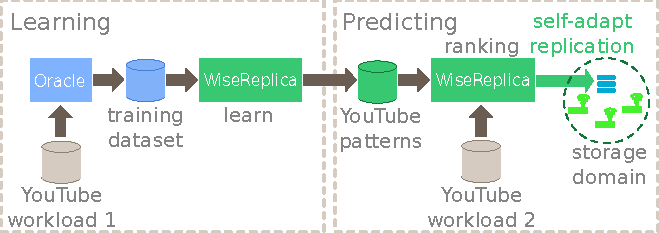
\includegraphics[width=.65\textwidth]{inputs/img/wisereplica_scheme}
  \caption{Framework for learning and predicting ranking of Internet videos .}
  \label{fig:model_scenario}
\end{figure}
